\section{UML}
\label{sc:UMLB}
UML ist heute eine der dominierenden Sprachen für die Modellierung von betrieblichen Anwendungs- bzw. Softwaresystemen. Der erste Kontakt zu UML besteht häufig darin, dass UML-Diagramme im Rahmen von Softwareprojekten zu erstellen, zu verstehen oder zu beurteilen sind. UML-Diagramme gelten als Standard bei objektorientierter Modellierung.
\subsection{Eignung}

Aus meiner persönlichen Sicht liegen die wesentlichen Vorteile bei dem Einsatz von UML in der breiten Unterstützung sämtlicher objektorientierter Grundsätze. Man kann an vielen Stellen ein und dasselbe Problem auf unterschiedliche Art und Weise lösen, ohne sich dabei durch die Vorgaben der Sprache eingeengt zu fühlen. Die Sprache lässt also den Softwareentwicklern den Freiraum, nach eigenen Vorstellungen zu modellieren. Besonders Vorteilhaft erscheint die Tatsache, dass UML auch die Erweiterungsmöglichkeiten durch eigene Sprachkonstrukte vorsieht (Metamodell), und damit wirklich jedem das Recht anbietet, den eigenen Notationsrahmen zu erschaffen. Diese Möglichkeit sollte aber nur in äußersten Notfällen (wenn es nicht anders geht) verwendet werden, da man sonst der Gefahr, sich vom Standard zu entfernen, entgegenläuft .\\
Weiterer Vorteil liegt in der Standardisierung der UML. Die  UML bietet eine fast perfekte Grundlage für die Kommunikation der verschiedenen Entwicklungsteams miteinander. Diagramme können nun nicht nur von den Fachleuten der Software –Firma , sondern auch von den außerhalb stehenden verstanden und verbessert werden. Lästiges  Einarbeiten in die verschiedenen Notationen entfällt, falls sich alle grundsätzlich an die UML halten. 
Weiterer Vorteil liegt in der zunehmenden Verbreitung der Unified Modeling Language. Die exakten Zahlen sind zwar noch schwer abzuschätzen, es zeichnet sich jedoch ein wachsender Trend für den Einsatz der UML ab.\\
Man kann die Vorteile von UML in vier wichtigste Punkte zusammenfassen wie folge:\\

- Die Vereinheitlichung der Terminologie und die Standardisierung der Notation
führen zu einer massiven Erleichterung der Verständigung zwischen allen
Beteiligten.\\
- Die UML wächst mit Ihren Anforderungen an die Modellierung. Sie können mit der
Erstellung einfacher Modelle beginnen, aber auch sehr komplexe Sachverhalte im
Detail modellieren, da die UML eine mächtige Modellierungssprache ist.\\
- Die UML baut auf bewährten und weit verbreiteten Ansätzen auf. Die UML wurde
nicht im Elfenbeinturm erstellt, sondern hat sich zu grossen Teilen aus der Praxis
und aus bestehenden Modellierungssprachen heraus entwickelt. Das gewährleistet
die Einsatzfähigkeit und Praxisnähe der UML.\\

\subsection{Uneignung}
Die Nachteile lassen sich nun wiederum aus dem Umfang der Sprache ableiten. UML ist sehr vielfältig, so dass auch am Anfang  sehr viel Aufwand für das Aneignen und Verstehen sämtlicher Sprachkonstrukte aufgebracht werden muss.\\ Außerdem wird man in der  Regel feststellen, dass viele Elemente sehr selten zum Einsatz kommen und damit eher als Ballast der Sprache angesehen werden. So habe ich in der Darstellung der UML Notation auf die Erläuterung der OCL Konstrukte (Object Constraint Language) verzichtet, obwohl OCL als formale Sprache zur Erweiterung der Semantik der UML Notation herangezogen werden kann. Damit lassen sich zwar Zusicherungen, Invarianten, Vor –und Nachbedingungen, Navigationspfade etc. kurz und aussagekräftig darstellen, aber man kann diese im begrenzten Maße auch durch UML Basiselemente beschreiben.\\
Speziell für die Entwicklung der Software für eingebettete Systeme lässt sich anmerken, dass UML eine objektorientierte Modellierungssprache ist. Sämtliche Konzepte von UML können nur dann ausgenutzt werden, wenn wirklich objektorientiert programmiert wird. Es macht wenig Sinn, objektorientiert zu modellieren , wenn  anschließend kein objektorientierter Code verwendet wird. Steht kein objektorientierter Compiler zur Verfügung, sollte man sich über den Einsatz anderer Werkzeuge und Spezifikationssprachen Gedanken machen. Man kann zwar im begrenzten Maße sämtliche objektorientierte Ansätze in den „strukturierten“ Code konvertieren (also z.B. von C++ nach C überführen), das Ergebnis lässt jedoch zu wünschen übrig, insbesondere leidet die Code- Qualität / Lesbarkeit darunter.\\

Man kann die Nachteile von UML in vier wichtigste Punkte zusammenfassen wie folge:\\
- Die neue Notation muss zuerst erlernt werden. Es fallen somit Schulungskosten an
und die Mitarbeiter müssen dafür Zeit aufwenden können.\\
- Im Bereich der Software-Unterstützung ist noch einiges zu tun, bis wirklich
benutzerfreundlich mit UML gearbeitet werden kann.\\
- Durch die Vereinheitlichung der Modellierungssprachen geht die Vielfalt und
Kreativität verloren. Kleine, vielleicht gute Modelle gehen verloren.\\
- Der Wettbewerb wird durch die Monopolisierung zerstört.
\subsection{Fazit}

Wir versuchen in diesem Abschnitt die Vorteile und Nachteile von UML zusammenfassen und einen Überblick darüber geben.


		
		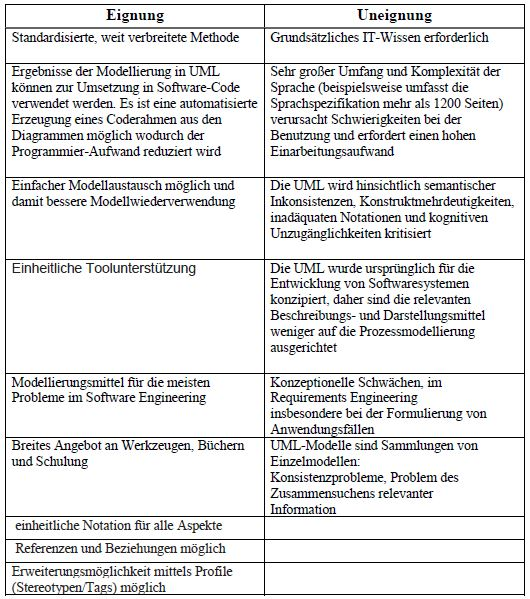
\includegraphics[scale=1]{Graphics/vornachteil.jpg} 
		\captionof{figure}{Eignung und Uneignung von UML}
		
		
		
